\PassOptionsToPackage{hyphens}{url}
\documentclass[10pt,a4paper]{article}

\usepackage[a4paper,margin=0.9in]{geometry}
\usepackage{fontspec}
\defaultfontfeatures{Ligatures=TeX}
% XeLaTeX/Overleaf setup:
% Upload these files into a `fonts/` folder in your Overleaf project:
%   fonts/GillSans.ttf
%   fonts/GillSans-Bold.ttf
%   fonts/GillSans-Italic.ttf
%   fonts/GillSans-BoldItalic.ttf
%
% If those files are present, the paper uses Gill Sans exactly from the
% uploaded fonts. Otherwise it falls back to Helvetica so the file still
% compiles.
\IfFileExists{fonts/GillSans.ttf}{
  \setmainfont[
    Path=fonts/,
    Extension=.ttf,
    UprightFont=*,
    BoldFont=*-Bold,
    ItalicFont=*-Italic,
    BoldItalicFont=*-BoldItalic
  ]{GillSans}
}{
  \setmainfont{Helvetica}
}
\usepackage{amsmath,amssymb}
\usepackage{graphicx}
\usepackage{booktabs}
\usepackage{array}
\usepackage{tabularx}
\usepackage{enumitem}
\usepackage{caption}
\usepackage{titlesec}
\usepackage{setspace}
\usepackage{natbib}
\usepackage{xurl}
\usepackage[hidelinks]{hyperref}

\setlength{\parindent}{0pt}
\setlength{\parskip}{0.22em}
\linespread{1.04}
\raggedbottom
\captionsetup{font=small,labelfont=bf}
\setlist[itemize]{leftmargin=1.4em,topsep=0.2em,itemsep=0.2em}

\titleformat{\section}
  {\centering\bfseries\normalsize}
  {\thesection}{0.7em}{}
\titlespacing*{\section}{0pt}{0.9em}{0.35em}

\titleformat{\subsection}
  {\bfseries\normalsize}
  {\thesubsection}{0.6em}{}
\titlespacing*{\subsection}{0pt}{0.65em}{0.25em}

\titleformat{\subsubsection}[runin]
  {\itshape}
  {\thesubsubsection}{0.5em}{}[.]
\titlespacing*{\subsubsection}{0pt}{0.45em}{0.4em}

\bibpunct{(}{)}{;}{a}{,}{,}
\setlength{\bibsep}{0pt}

\newcommand{\figsource}[1]{\caption*{\footnotesize\textit{Source: #1.}}}
\newcommand{\tabsource}[1]{\caption*{\footnotesize\textit{Source: #1.}}}

\begin{document}
\pagestyle{plain}

\begin{center}
{\fontsize{20}{24}\selectfont\bfseries Digital Inclusion and Circular Economy Behavior in Indian States: A Digital Circularity Index and Explainable XGBoost Analysis\par}
\vspace{0.6cm}
{\large\bfseries Suresh Kumar Chelliah, Shreya Srivastava and Yash Chauhan\par}
\vspace{0.15cm}
{\normalsize Department of Computational Intelligence, SRM Institute of Science \& Technology, Kattankulathur, Tamil Nadu, India\par}
{\normalsize sureshkc@srmist.edu.in; ss1371@srmist.edu.in; yc0810@srmist.edu.in\par}
\end{center}

\textbf{Abstract:} India is pursuing two large national transitions at the same time: rapid digital expansion through broadband, mobile connectivity and platform-based payments, and a circular-economy agenda aimed at reducing waste, improving resource efficiency and strengthening environmental performance. Although both agendas are policy priorities, they are usually examined separately. This paper studies whether they are linked at the state level. Using seven official and policy-relevant data sources, we compile a harmonised dataset for 16 Indian states and construct three composite indicators: the Digital Access Score (DAS), the Circular Economy Behavior Score (CEBS) and the Digital Circularity Index (DCI). The analysis combines descriptive comparison, ordinary least squares regression, non-parametric and permutation-based robustness checks, mediation and threshold testing, leak-free nested cross-validation, SHAP-based explainability and K-Means clustering. Across methods, the central pattern is consistent: states with stronger digital access also tend to show stronger circular-economy performance. The baseline OLS model reports a strong positive association between DAS and CEBS ($r=0.781$, $p<0.001$), while alternative rank-based and resampling checks preserve the result. Tele-density emerges as the most influential variable across both statistical and machine-learning analyses, whereas UPI adoption does not mediate the relationship. Nested leave-one-out cross-validation confirms that predictive performance survives stricter out-of-sample testing, with XGBoost delivering the strongest leak-free result ($R^2=0.511$). Clustering further separates the states into digitally stronger and digitally lagging groups, revealing a substantial gap in average DCI. The findings suggest that digital inclusion is not only a financial or communications issue but also a governance and sustainability capacity issue. Policy design in India should therefore treat digital infrastructure and circular-economy outcomes as interconnected development priorities rather than parallel policy tracks.

\textbf{Keywords:} circular economy; digital circularity index (DCI); digital inclusion; explainable machine learning; Indian states; XGBoost

\section{Introduction}

India's recent development trajectory has been shaped by the simultaneous spread of digital infrastructure and the growing policy importance of the circular economy. Monthly UPI transactions now exceed 14 billion \citep{npci2025}, national tele-density remains above 85\% \citep{trai2024}, and Digital India has expanded broadband and mobile access into increasingly diverse regional contexts. At the same time, India faces mounting waste-management pressures, including e-waste, urban waste and resource-use inefficiency, while national policy institutions have begun framing circularity as a core long-term growth strategy \citep{cpcb2023,nitiCE2021}.

Despite this overlap in policy timing, the two agendas are usually analysed in isolation. Research on digital inclusion in India concentrates mainly on access, payments and growth \citep{meity2023}, while circular-economy research focuses on waste systems, environmental governance and industrial transitions \citep{geissdoerfer2017}. State-level evidence linking digital access with circular-economy outcomes remains limited. This paper addresses that gap by constructing a state-level Digital Circularity Index from seven public data sources and testing whether digitally stronger states also perform better on selected circular-economy indicators.

The study evaluates three hypotheses. H1 states that states with higher Digital Access Scores will also have higher CE Behavior Scores. H2 states that UPI adoption mediates the relationship between digital access and CE behavior. H3 states that there is a tele-density threshold beyond which CE behavior improves more sharply.

\section{Literature Review}

Digital inclusion in India has advanced rapidly, but unevenly. Tele-density and digital payments have expanded across the country, yet large regional gaps remain between higher-capacity states and states with weaker infrastructure or lower income levels \citep{trai2024,npci2025}. Existing literature generally treats these developments as drivers of financial inclusion, efficiency and service access \citep{meity2023}. Broader ICT-for-development scholarship, however, argues that digital systems also shape governance, information flows and institutional capacity, implying that their effects may extend into environmental management and sustainability outcomes \citep{avgerou2010,heeks2017}.

Circular-economy research highlights a similar implementation gap. The concept has moved from global advocacy into Indian policy planning, especially through NITI Aayog's sector-based framework \citep{emf2013,nitiCE2021}. Yet state performance remains uneven, formal e-waste processing is limited relative to total waste generation, and SDG-linked environmental outcomes still vary substantially \citep{cpcb2023,nitiSDG2024}. Taken together, these strands suggest a plausible connection: states with stronger digital access may be better positioned to coordinate reporting, traceability, administration and circular-economy behavior. This paper tests that possibility directly.

\section{Methodology}

\subsection{Research Design and Data}

The study uses a cross-sectional design based on 16 Indian states with complete observations across all selected inputs. We retain only states that are comparable across every source, prioritising traceability over larger sample size. The final dataset combines nine raw and six derived variables.

\begin{table}[htbp]
\centering
\caption{Data Sources and Core Variables}
\label{tab:data_sources_24}
\small
\begin{tabularx}{\textwidth}{@{}>{\raggedright\arraybackslash}p{3.0cm}>{\raggedright\arraybackslash}X>{\raggedright\arraybackslash}p{1.5cm}@{}}
\toprule
\textbf{Source} & \textbf{Variable} & \textbf{Year} \\
\midrule
TRAI & Tele-density (\%) & 2024 \\
RBI & Per capita NSDP (INR) & 2023--24 \\
NITI Aayog & SDG Index Score & 2023--24 \\
NPCI/Dataful Insights & UPI transactions per capita & 2024--25 \\
CPCB & E-waste processed (tonnes) & 2021--22 \\
Census of India & Literacy rate (\%) & 2011 \\
Census of India & Urban population (\%) & 2011 \\
\bottomrule
\end{tabularx}
\tabsource{Compiled from TRAI, RBI, NITI Aayog, NPCI/Dataful Insights, CPCB and Census of India}
\end{table}

\subsection{Composite Index Construction}

Each raw variable is first rescaled to a 0--100 range using min--max normalisation:
\begin{equation}
\hat{x}_i=\frac{x_i-x_{\min}}{x_{\max}-x_{\min}}\times 100
\end{equation}

The Digital Access Score is defined as:
\begin{equation}
DAS = 0.40\hat{T}_d + 0.30\hat{U}_{pc} + 0.30\hat{N}_{pc}
\end{equation}
where $\hat{T}_d$ is tele-density, $\hat{U}_{pc}$ is UPI transactions per capita and $\hat{N}_{pc}$ is per capita NSDP after normalisation.

The Circular Economy Behavior Score is defined as:
\begin{equation}
CEBS = 0.35\hat{E}_{pc} + 0.40S_{sdg} + 0.25\hat{N}_{pc}
\end{equation}
where $\hat{E}_{pc}$ is normalised e-waste processed per capita and $S_{sdg}$ is the SDG Index score. The Digital Circularity Index then combines both dimensions multiplicatively:
\begin{equation}
DCI=\frac{DAS \times CEBS}{100}
\end{equation}

\subsection{Analytical Strategy}

H1 is tested using a bivariate OLS model of CEBS on DAS, followed by HC3 robust errors, permutation tests, bootstrap intervals and rank-based correlations. H2 is assessed using the Baron and Kenny mediation framework with a Sobel test \citep{baron1986}. H3 is examined through piecewise regression with grid-searched breakpoint selection. To assess predictive stability, we compare seven models under leave-one-out cross-validation and then apply a stricter nested leave-one-out design. XGBoost is interpreted using SHAP values \citep{lundberg2017}, and K-Means clustering is used to identify state typologies.

\section{Results and Discussion}

\subsection{Descriptive Patterns}

The descriptive evidence already suggests a strong divide between digitally advanced and digitally lagging states. Haryana records the highest DCI (72.97), Karnataka posts the highest DAS (94.40), and Bihar ranks lowest across all three composite indicators. Figure~\ref{fig:dci_ranking_24} summarises the state-level spread.

\begin{figure}[htbp]
\centering
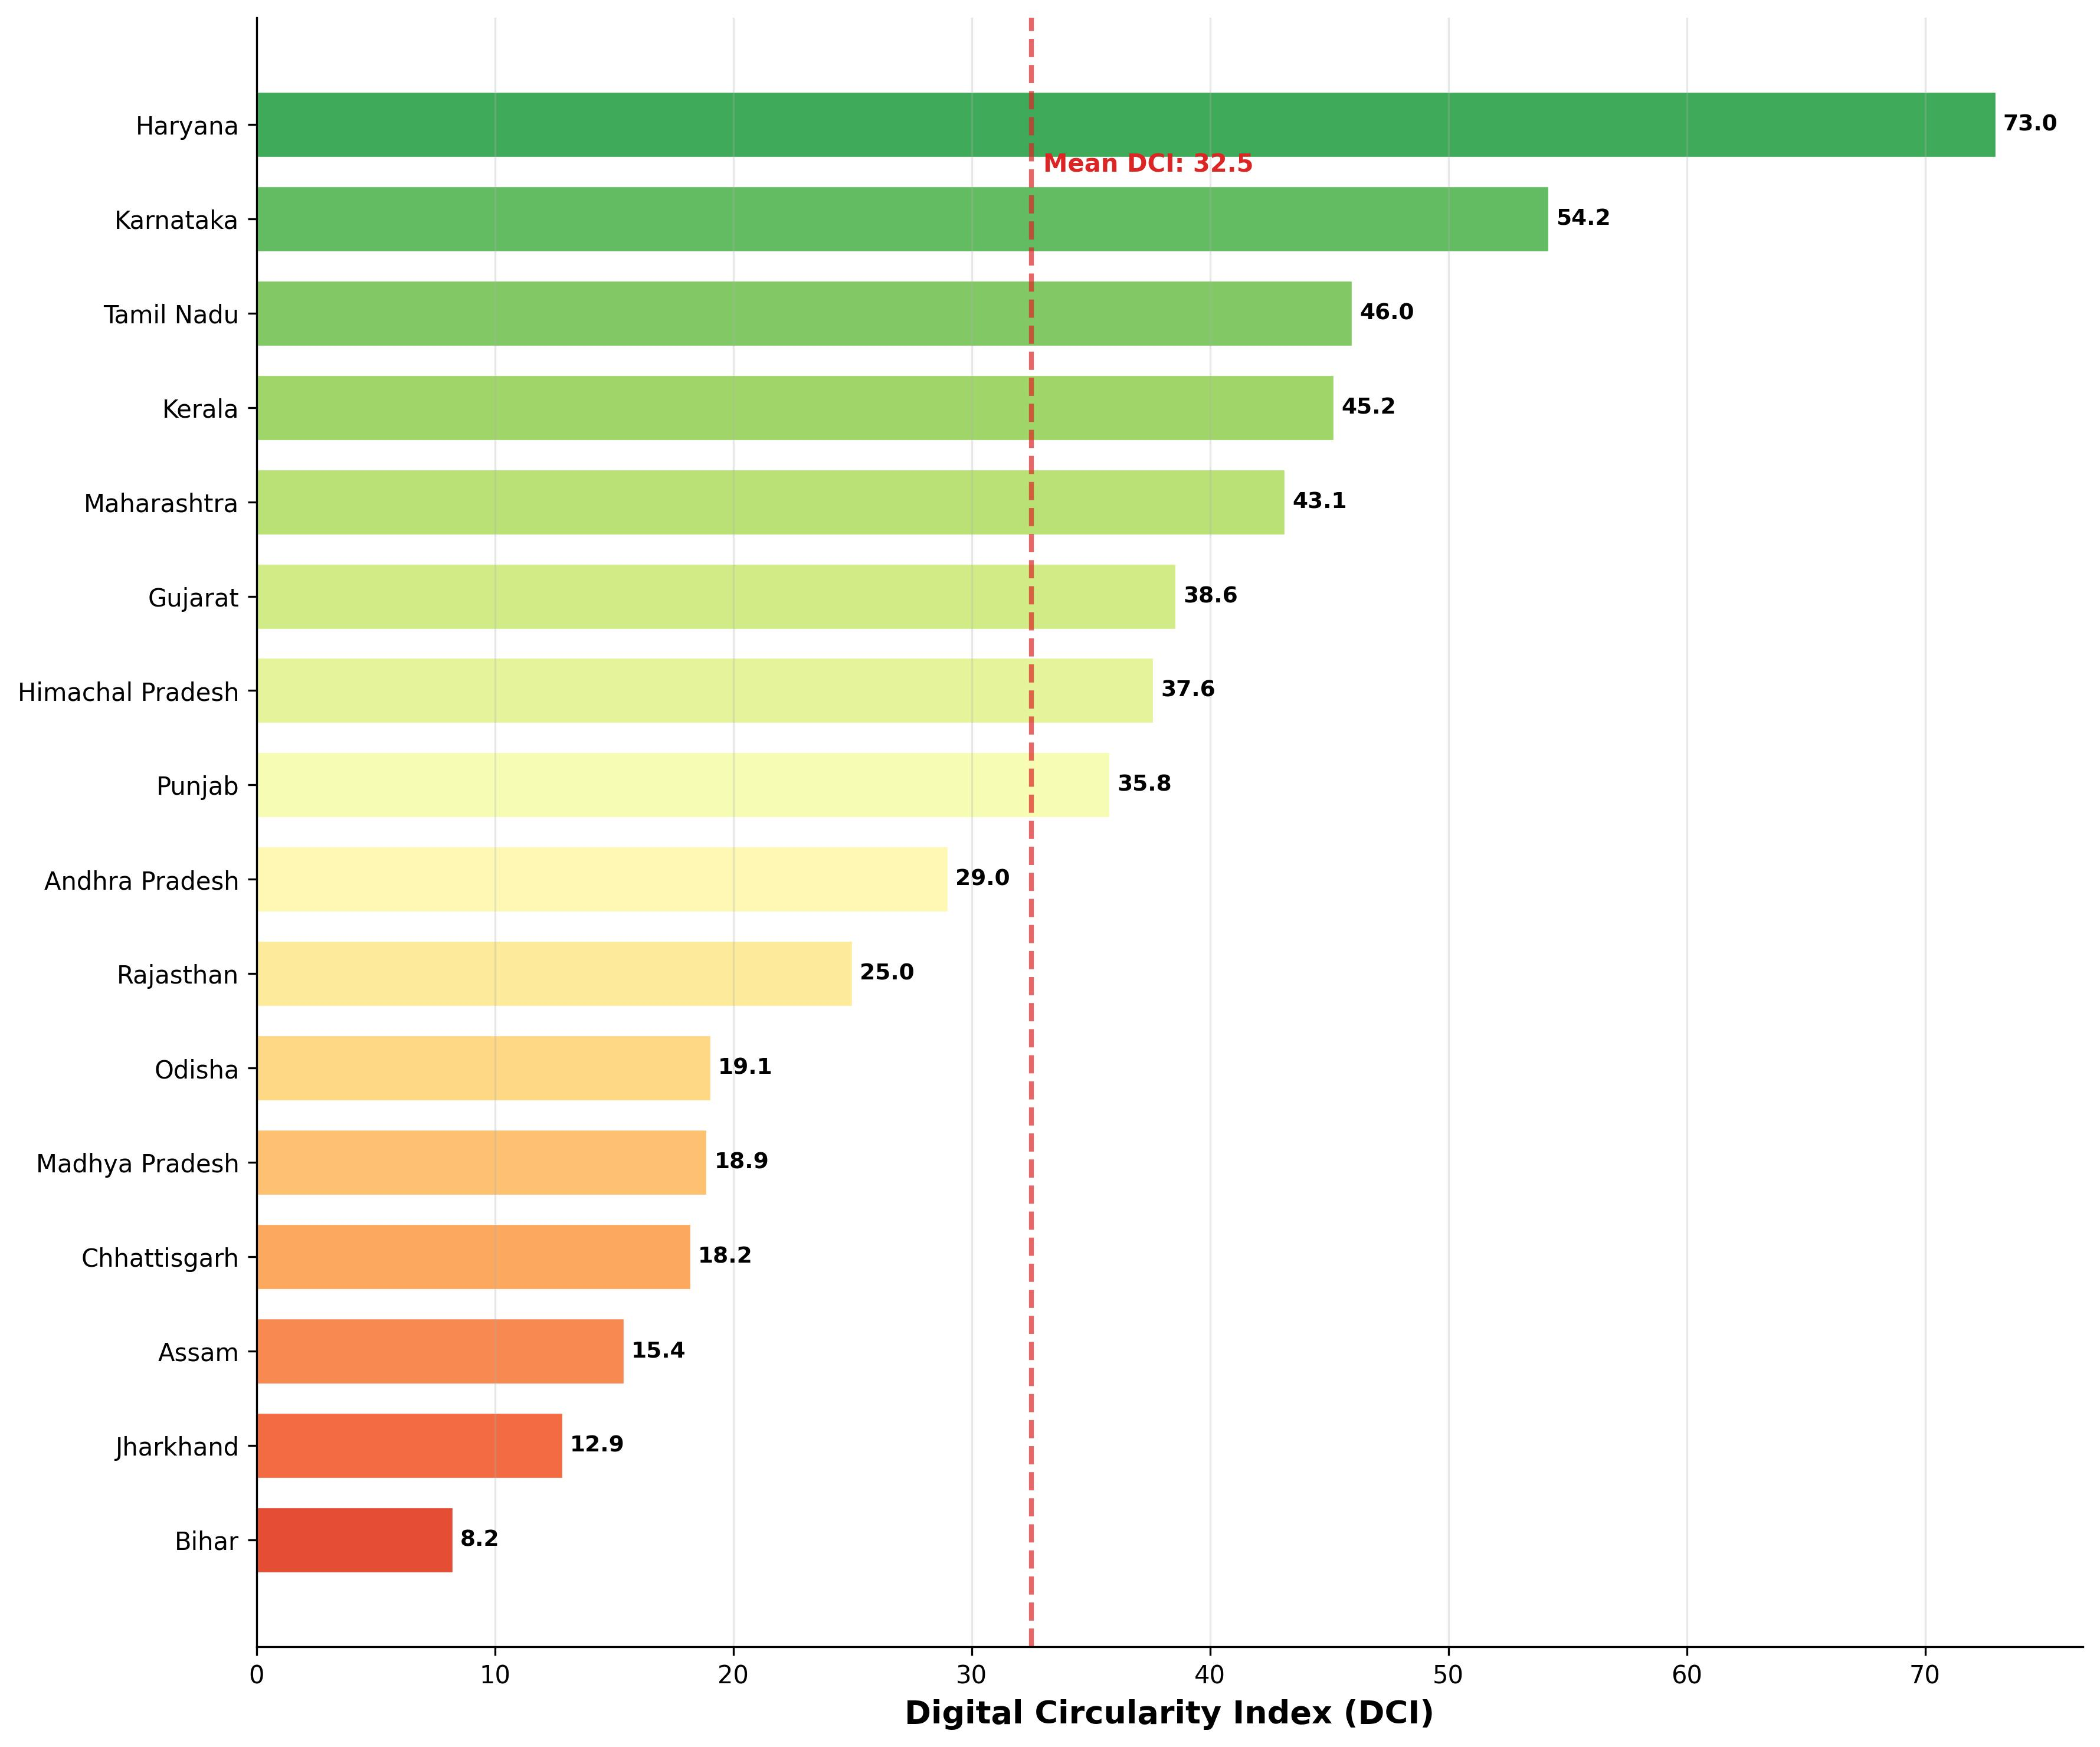
\includegraphics[width=0.82\textwidth]{figures/fig3_dci_ranking.jpg}
\caption{Digital Circularity Index ranking across 16 Indian states.}
\label{fig:dci_ranking_24}
\figsource{Authors' analysis based on the compiled state-level dataset}
\end{figure}

\subsection{Regression, Robustness and Mechanisms}

The baseline OLS result supports H1. A one-point increase in DAS is associated with a 0.551-point increase in CEBS, and the model explains 61\% of the observed variation. Figure~\ref{fig:scatter_24} shows the positive association, while Table~\ref{tab:core_results_24} summarises the main statistical findings. The relationship remains significant under HC3 robust inference, permutation testing and rank-based correlation, which reduces concern that the result is being driven only by distributional assumptions.

\begin{figure}[htbp]
\centering
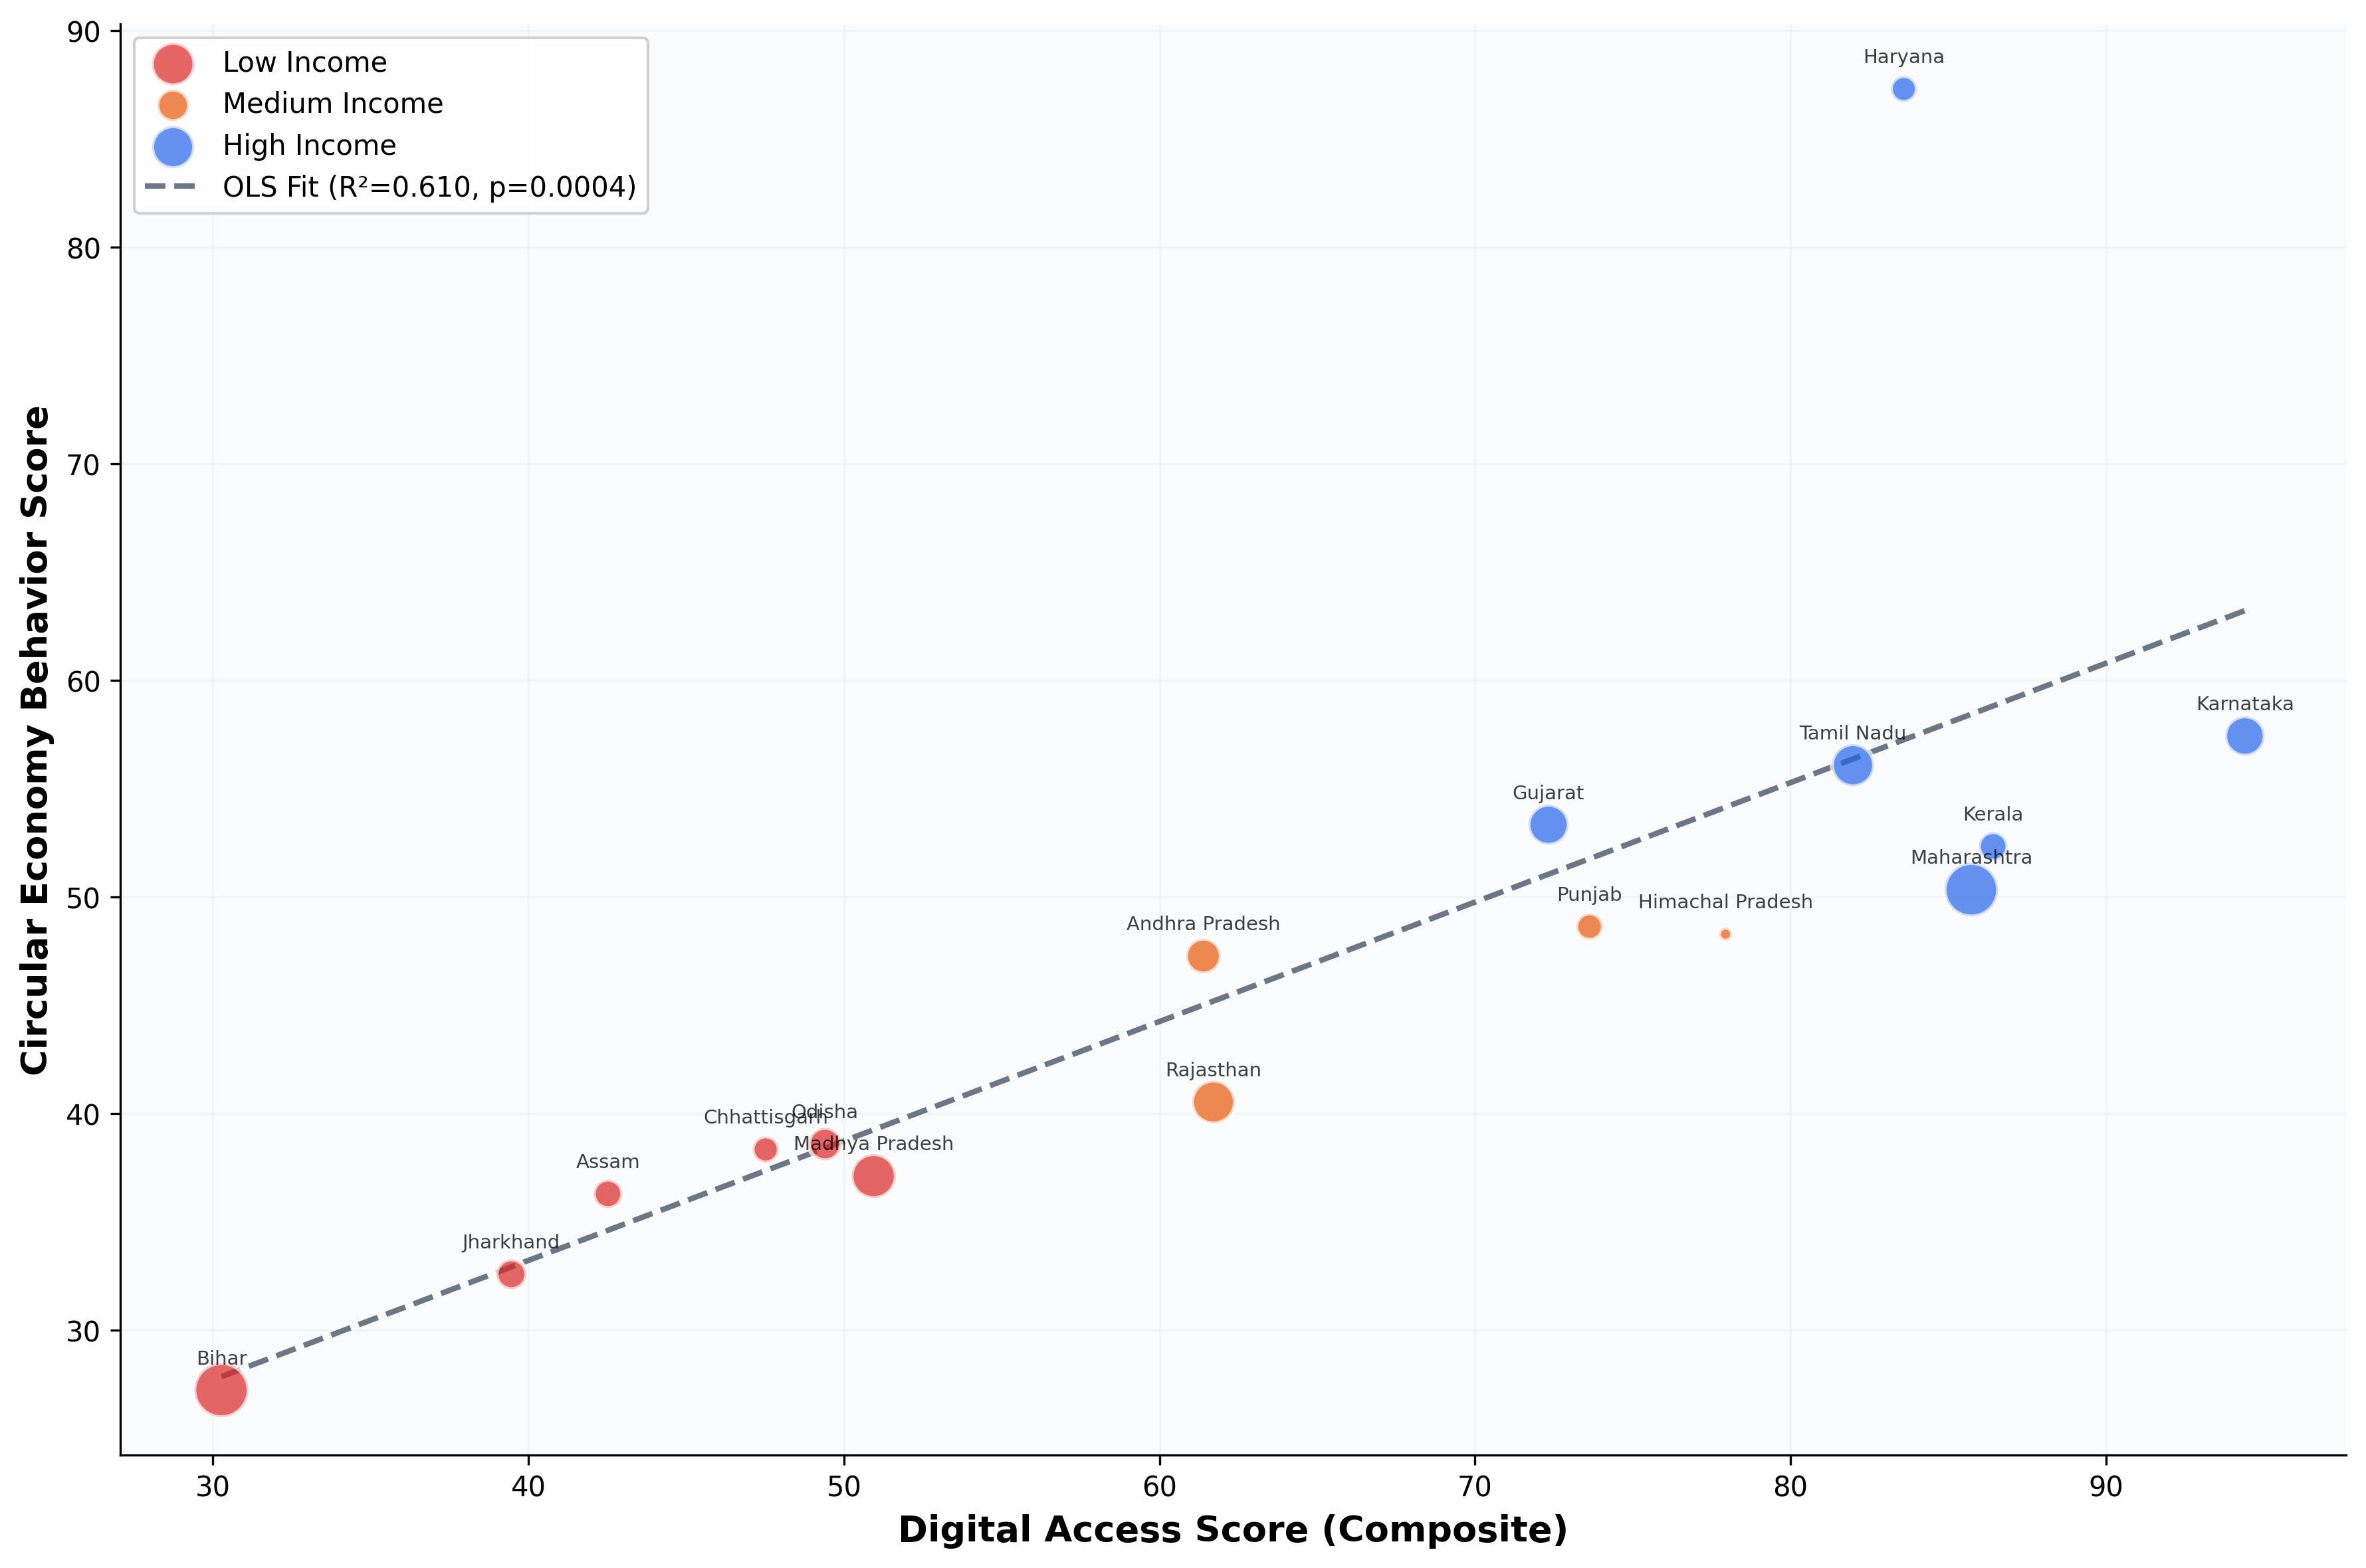
\includegraphics[width=0.75\textwidth]{figures/fig2_digital_vs_ce_scatter.jpg}
\caption{Digital Access Score and CE Behavior Score across the 16-state sample.}
\label{fig:scatter_24}
\figsource{Authors' analysis based on the compiled state-level dataset}
\end{figure}

\begin{table}[htbp]
\centering
\caption{Core Statistical Results}
\label{tab:core_results_24}
\small
\begin{tabularx}{\textwidth}{@{}>{\raggedright\arraybackslash}X>{\raggedright\arraybackslash}p{2.2cm}>{\raggedright\arraybackslash}p{3.0cm}@{}}
\toprule
\textbf{Test or Model} & \textbf{Value} & \textbf{Interpretation} \\
\midrule
OLS association (H1) & $R^2=0.610$; $\beta_1=0.551$; $p=0.000352$ & Strong positive relationship between DAS and CEBS \\
Pearson correlation & $r=0.781$ & Substantively large positive association \\
Spearman correlation & $\rho=0.912$; $p<0.001$ & Rank-order relationship remains strong \\
HC3 robust inference & $p=0.000011$ & Result remains significant under heteroskedasticity-robust errors \\
Permutation test & $p=0.0001$ & Association is unlikely under random reassignment \\
Mediation via UPI (H2) & Sobel $z=-0.241$; $p=0.810$ & No evidence that UPI mediates the main relationship \\
Threshold analysis (H3) & Breakpoint $=118.77\%$ tele-density & CE performance rises sharply up to the threshold, but evidence above it is based on very few states \\
\bottomrule
\end{tabularx}
\tabsource{Authors' analysis}
\end{table}

The mediation result does not support H2. Once DAS is already in the model, UPI adoption contributes little explanatory value and the indirect path is not significant. By contrast, the threshold analysis offers qualified support for H3. CE performance improves strongly up to roughly 119\% tele-density, but the post-threshold slope is estimated from only a small number of states, so the breakpoint should be interpreted cautiously.

\subsection{Predictive Validation and Explainability}

The predictive analysis confirms that the pattern is not limited to in-sample fitting. In standard leave-one-out cross-validation, ElasticNet performs best among the digital-only models ($R^2=0.364$), while Lasso performs best in the full-feature comparison ($R^2=0.568$). Under the stricter nested leave-one-out setup, XGBoost achieves the strongest leak-free result ($R^2=0.511$), narrowly outperforming Random Forest. SHAP analysis then shows that tele-density and per capita NSDP are the two most influential variables, whereas UPI contributes far less than expected. Figure~\ref{fig:shap_24} visualises that global importance pattern.

\begin{figure}[htbp]
\centering
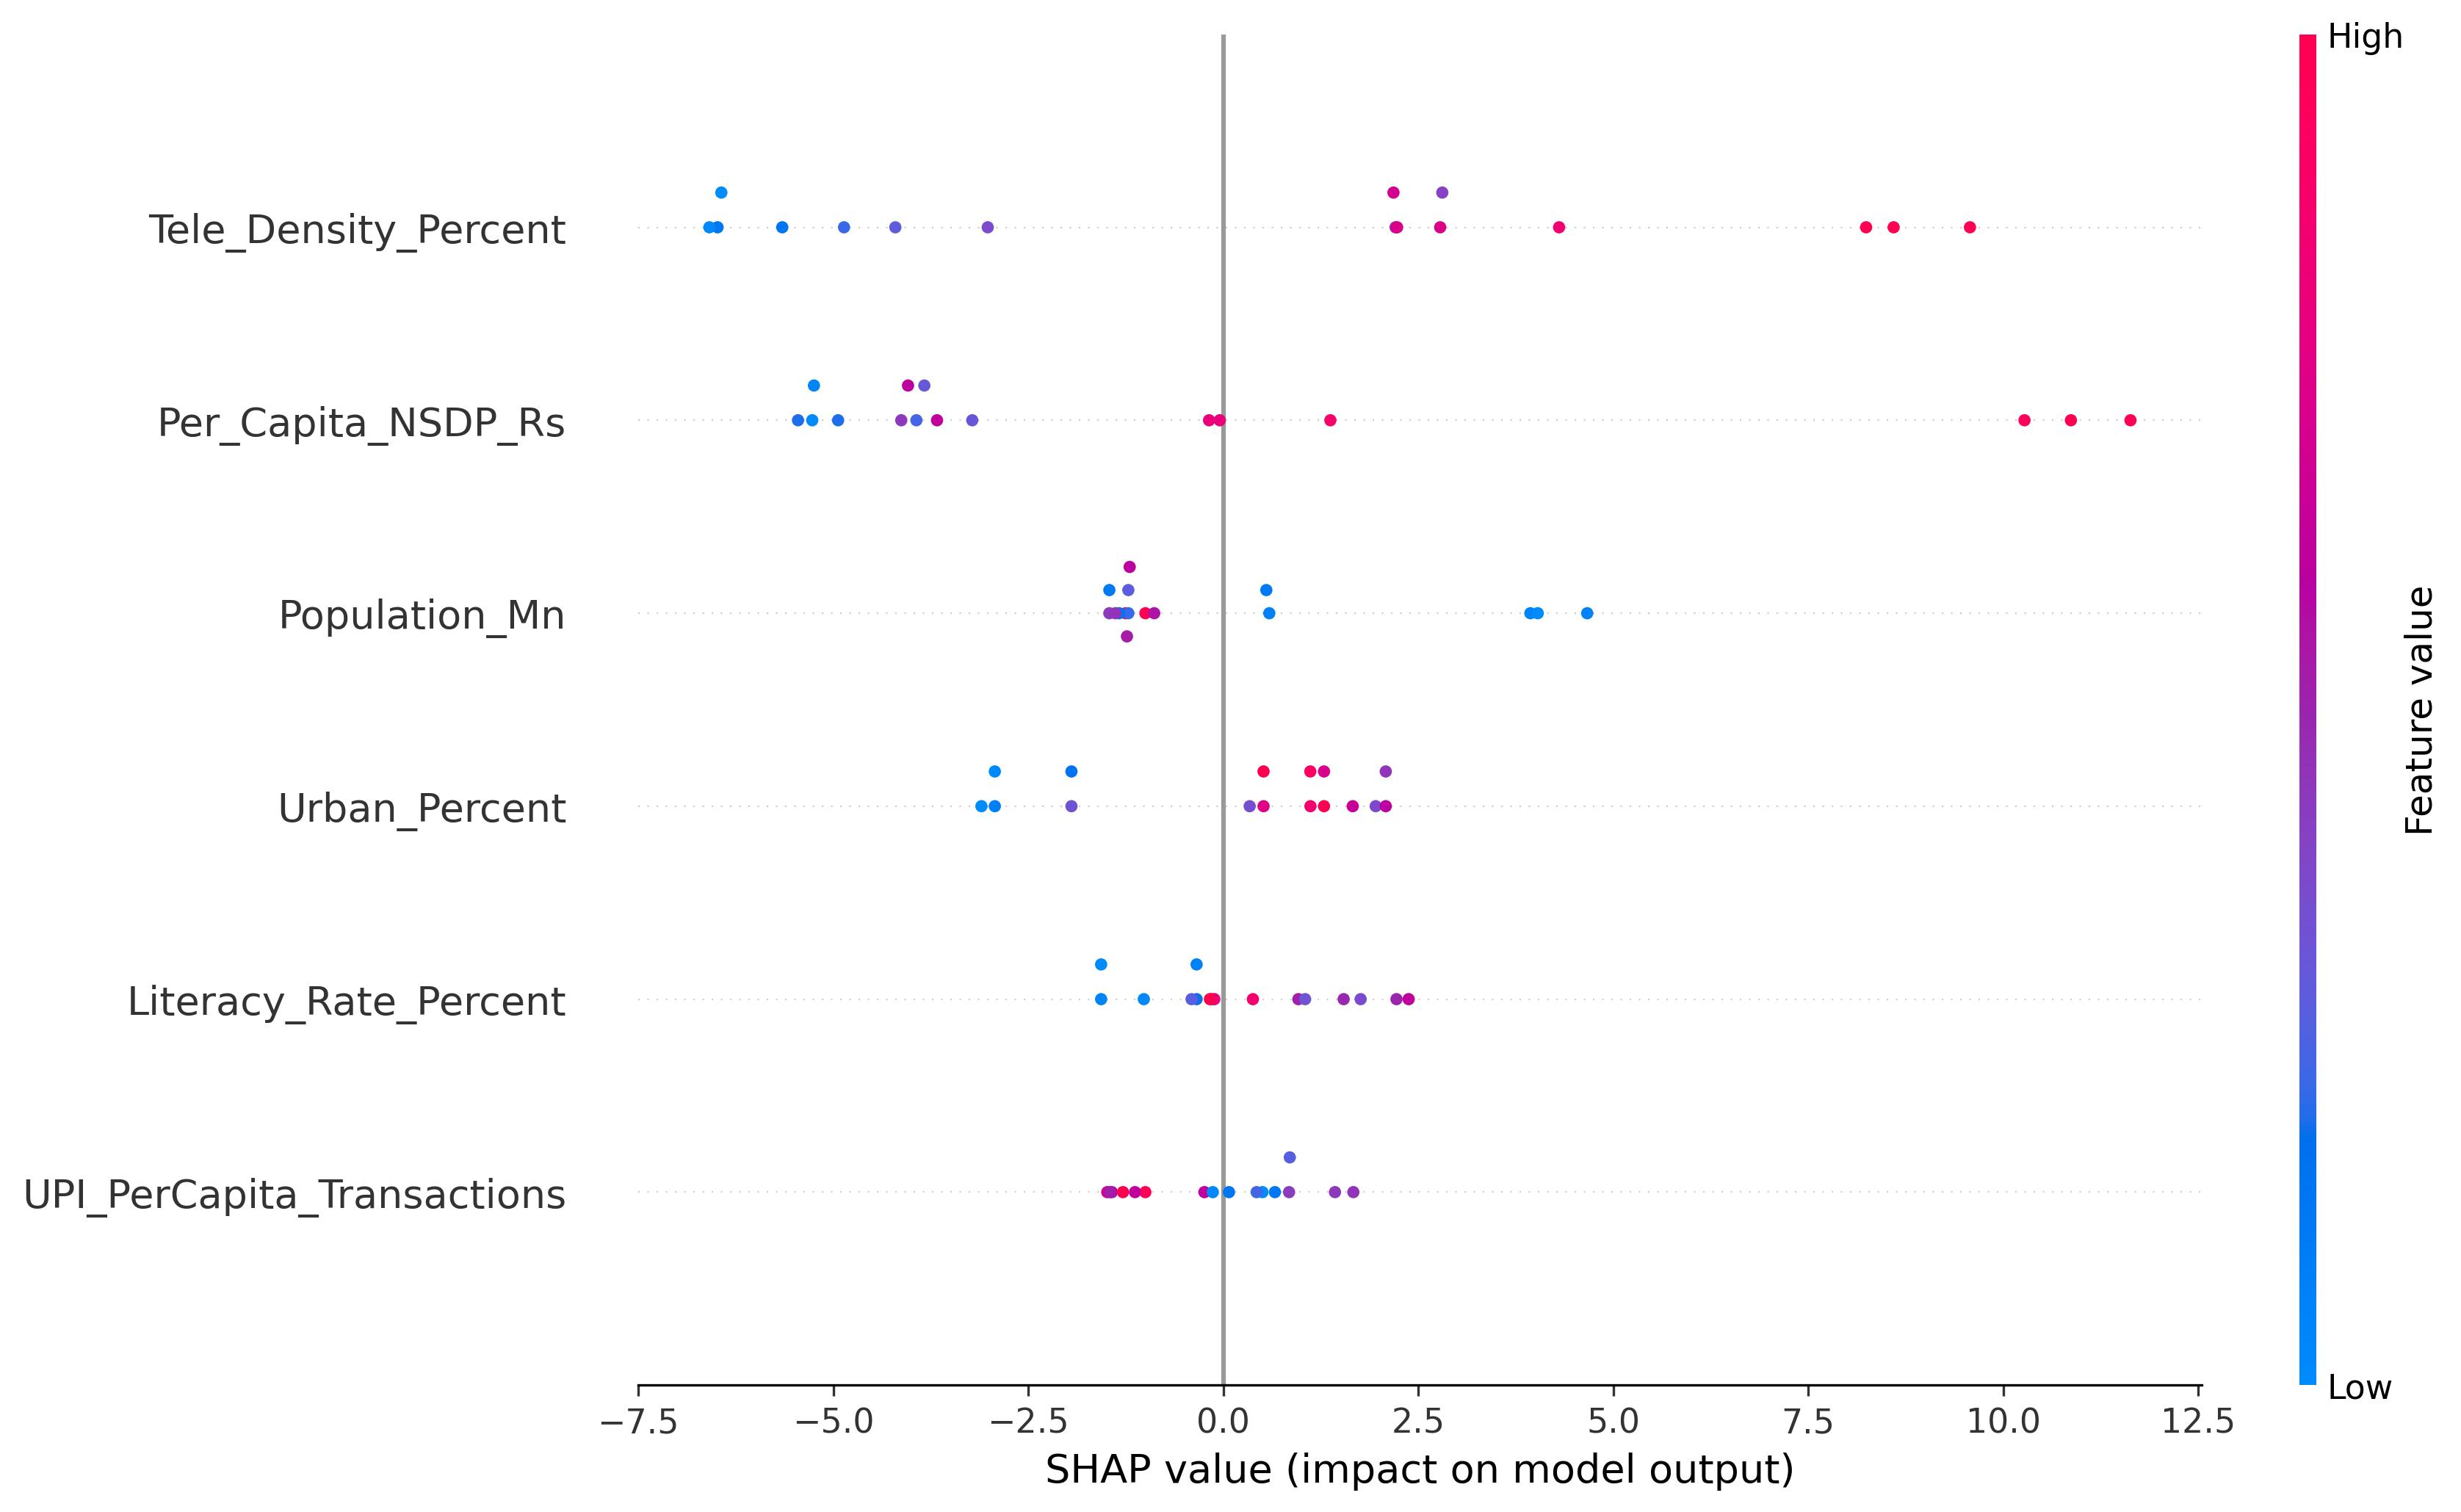
\includegraphics[width=0.80\textwidth]{figures/fig17_shap_beeswarm.jpg}
\caption{SHAP beeswarm plot for the nested XGBoost model.}
\label{fig:shap_24}
\figsource{Authors' analysis}
\end{figure}

\begin{table}[htbp]
\centering
\caption{Predictive, Explainability and Clustering Summary}
\label{tab:ml_results_24}
\small
\begin{tabularx}{\textwidth}{@{}>{\raggedright\arraybackslash}X>{\raggedright\arraybackslash}p{2.5cm}>{\raggedright\arraybackslash}X@{}}
\toprule
\textbf{Analysis} & \textbf{Key Result} & \textbf{Interpretation} \\
\midrule
Best digital-only LOO-CV model & ElasticNet, $R^2=0.364$ & Digital-access variables alone retain meaningful out-of-sample predictive value \\
Best full-model LOO-CV model & Lasso, $R^2=0.568$ & Predictive performance remains close to the main OLS result \\
Best nested LOO-CV model & XGBoost, $R^2=0.511$ & Main signal survives stricter leak-free evaluation \\
Top SHAP drivers & Tele-density; per capita NSDP & Infrastructure and economic capacity dominate the model explanation \\
K-Means typology & Two clusters; mean DCI 46.7 vs.\ 18.3 & States separate into digital leaders and emerging states with a large circularity gap \\
Extended-sample check & $n=21$; $r=0.963$ & Removing e-waste from CEBS strengthens rather than weakens the pattern \\
\bottomrule
\end{tabularx}
\tabsource{Authors' analysis}
\end{table}

The clustering result adds a policy-relevant interpretation. Rather than a smooth national gradient, the data point to two broad development settings. One cluster combines higher digital access with stronger CE outcomes, while the other remains weaker on both. This supports the view that digital infrastructure, administrative capacity and sustainability behavior are linked in practice. The evidence also indicates that tele-density matters more than digital payments alone, suggesting that broad infrastructural reach is more consequential than transaction activity by itself.

\subsection{Implications and Limitations}

The findings imply that digital inclusion and circular-economy strategy should not be treated as isolated policy domains. In lagging states, connectivity investment may also function as environmental capacity-building by improving reporting, traceability, service delivery and administrative coordination. At the same time, the study remains limited by its small cross-sectional sample, the use of 2011 Census controls, the inclusion of NSDP in both composite scores and the compression of within-state variation into state averages. The results therefore establish a robust association, not a causal effect. Future work should extend the framework using district-level or panel data and a broader set of circular-economy indicators.

\section{Conclusion}

This paper develops a Digital Circularity Index for 16 Indian states and shows that digital access is consistently associated with stronger circular-economy behavior. The result holds across regression, robustness checks, predictive validation and explainability analysis. Tele-density and economic capacity emerge as the most important drivers, while UPI adoption does not mediate the main relationship. The broader implication is straightforward: in India, digital inclusion should be understood not only as a communications or payments issue, but also as part of the institutional foundation for better sustainability outcomes.

\section*{Acknowledgment}

The authors acknowledge the Telecom Regulatory Authority of India, the Reserve Bank of India, NITI Aayog, the National Payments Corporation of India, the Central Pollution Control Board and the Census of India for maintaining the public datasets used in this study.

\clearpage
\section*{References}
\begin{spacing}{1.05}
\begin{thebibliography}{00}

\bibitem[Avgerou(2010)]{avgerou2010}
Avgerou, C. (2010) `Discourses on ICT and development', \textit{Information Technologies \& International Development}, 6(3), pp. 1--18.

\bibitem[Baron and Kenny(1986)]{baron1986}
Baron, R.M. and Kenny, D.A. (1986) `The moderator-mediator variable distinction in social psychological research: Conceptual, strategic, and statistical considerations', \textit{Journal of Personality and Social Psychology}, 51(6), pp. 1173--1182.

\bibitem[Census of India(2011)]{census2011}
Census of India (2011) \textit{Primary Census Abstract: Literacy Rate, Level of Urbanization, Population} [online]. Available at: \url{https://censusindia.gov.in} (Accessed: 23 April 2026).

\bibitem[CPCB(2023)]{cpcb2023}
CPCB (2023) \textit{Annual Report on Implementation of E-Waste (Management) Rules, 2016 for FY 2021--22} [online]. New Delhi: Central Pollution Control Board. Available at: \url{https://cpcb.nic.in/e-waste/} (Accessed: 23 April 2026).

\bibitem[Dataful Insights(2026)]{dataful2026}
Dataful Insights (2026) `Here is how UPI usage differs across Indian states' [online]. Available at: \url{https://insights.dataful.in/articles/here-is-how-upi-usage-differs-across-indian-states} (Accessed: 23 April 2026).

\bibitem[Ellen MacArthur Foundation(2013)]{emf2013}
Ellen MacArthur Foundation (2013) \textit{Towards the Circular Economy: Economic and Business Rationale for an Accelerated Transition}. Cowes: Ellen MacArthur Foundation.

\bibitem[Geissdoerfer et al.(2017)]{geissdoerfer2017}
Geissdoerfer, M., Savaget, P., Bocken, N.M.P. and Hultink, E.J. (2017) `The circular economy: a new sustainability paradigm?', \textit{Journal of Cleaner Production}, 143, pp. 757--768.

\bibitem[Heeks(2017)]{heeks2017}
Heeks, R. (2017) \textit{Information and Communication Technology for Development (ICT4D)}. Abingdon: Routledge.

\bibitem[Lundberg and Lee(2017)]{lundberg2017}
Lundberg, S.M. and Lee, S.-I. (2017) `A unified approach to interpreting model predictions'. In: \textit{Advances in Neural Information Processing Systems}, 30.

\bibitem[Ministry of Electronics \& IT(2023)]{meity2023}
Ministry of Electronics \& IT (2023) \textit{Digital India Programme: Progress and Initiatives} [online]. Available at: \url{https://digitalindia.gov.in} (Accessed: 23 April 2026).

\bibitem[NITI Aayog(2021)]{nitiCE2021}
NITI Aayog (2021) \textit{Circular Economy in India: Rethinking Growth for Long-Term Prosperity}. New Delhi: Government of India.

\bibitem[NITI Aayog(2024)]{nitiSDG2024}
NITI Aayog (2024) \textit{SDG India Index \& Dashboard 2023--24}. 4th edn [online]. New Delhi: Government of India. Available at: \url{https://sdgindiaindex.niti.gov.in} (Accessed: 23 April 2026).

\bibitem[NPCI(2025)]{npci2025}
NPCI (2025) \textit{UPI Product Statistics (Monthly)} [online]. Mumbai: National Payments Corporation of India. Available at: \url{https://www.npci.org.in/what-we-do/upi/product-statistics} (Accessed: 23 April 2026).

\bibitem[RBI(2025)]{rbi2025}
RBI (2025) \textit{Handbook of Statistics on Indian Economy 2024--25, Table 9: Per Capita Net State Domestic Product} [online]. Mumbai: Reserve Bank of India. Available at: \url{https://www.rbi.org.in/scripts/AnnualPublications.aspx?head=Handbook+of+Statistics+on+Indian+Economy&lang=en} (Accessed: 23 April 2026).

\bibitem[TRAI(2024)]{trai2024}
TRAI (2024) \textit{Indian Telecom Services Performance Indicators Report: April--June 2024} [online]. New Delhi: Telecom Regulatory Authority of India. Available at: \url{https://www.trai.gov.in/sites/default/files/2024-09/IndicatorReport1oct09.pdf} (Accessed: 23 April 2026).

\end{thebibliography}
\end{spacing}

\end{document}
